% Trabalho de Política Habitacional
%
% Abaixo seguem orientações originais do modelo utilizado.
%
% Siga para o conteúdo do trabalho descendo até a linha 867
%
% ==============================================================
%
% Modelo para monografia de final de curso, em conformidade
% com normas da ABNT implementadas pelo projeto abntex2.
%
% Este arquivo é fortemente baseado em exemplo distribuído no
% mesmo projeto. O projeto abntex2 pode ser acessado pela página
% http://abntex2.googlecode.com/
%
% Este arquivo pode ser rodado tanto com o pdflatex quanto com
% o lualatex.  Como contém referências bibliográficas a serem
% processadas pelo programa bibtex, este programa deve ser
% executado. Em resumo, a ordem de execução deve ser:
% rodar primeiro o pdflatex (ou o lualatex), depois o bibtex e,
% a seguir, o pdflatex (ou o lualatex ) novamente mais duas vezes,
% para assegurar que todas as referências bibliográficas e 
% citações estejam atualizadas.
%
% Para adaptar os textos para uso pessoal, usar os comandos
% imediatamente antes do \begin{document} (iniciando com o
% comando \titulo).  
%
% Este modelo está adaptado para monografias de final de curso
% em matemática da UFRJ, mas, com o uso das variáveis, pode ser
% usado para outros tipos de trabalho (mestrado, doutorado),
% outros cursos, universidades etc.  Caso a adaptação das
% variáveis não seja suficiente, pode-se alterar os comandos
% imprimircapa, imprimirfolhaderosto e imprimiraprovação, 
% fazendo as alterações necessárias.  Como os comandos definidos
% neste texto usam somente LaTeX, a sua adaptação deve ser 
% simples, bastando algum conhecimento de LaTeX.
%
% O restante do preâmbulo provavelmente  não necessitará ser
% alterado, a menos, eventualmente, das opções de chamada da
% classe abntex2, que estão definidas a seguir.
% 
\documentclass[ 
% -- opções da classe memoir que é a classe base da abntex2 --
% tamanho da fonte
12pt,
% capítulos começam em pág ímpar. Insere pág vazia, se preciso
openright,
% para imprimir uma página por folha ou visualização em video 
oneside,
% frente e verso. Margens das pag. ímpares diferem das pares.
%  twoside,
% tamanho do papel. 
a4paper,
% Caio - Ocultando bordas horríveis em hiperligações
hidelinks,
% -- opções da classe abntex2 --
% títulos de capítulos convertidos em letras maiúsculas
%  chapter=TITLE,
% títulos de seções convertidos em letras maiúsculas
%  section=TITLE,
% títulos de subseções convertidos em letras maiúsculas
%  subsection=TITLE,
% títulos de subsubseções convertidos em letras maiúsculas
%  subsubsection=TITLE,
% -- opções do pacote babel --
english,   % idioma adicional para hifenização
portuguese,   % o último idioma é o principal do documento
oldfontcommands,
]{abntex2}
%
% ==============================================================
%
% --------------------------------------------------------------
% Adicionando pacotes para recursos adicionais e defindo opções
% pertinentes
% --------------------------------------------------------------
%
% cabeçalho comum para uso com lualatex ou pdflatex
\usepackage{ifluatex}
% opções para uso com o lualatex
\ifluatex
\usepackage{fontspec}
\defaultfontfeatures{Ligatures=TeX}
% o fonte small caps é diferente no latin modern
\fontspec[SmallCapsFont={Latin Modern Roman Caps}]{Latin Modern Roman}
% pacotes da AMS 
\usepackage{amsmath,amsthm} 
% pacote para fonte específico para símbolos matemáticos
\usepackage{unicode-math}
\setmathfont{Latin Modern Math}
% latin modern tem simbolos de mathbb muito feios.
%  Trocar o fonte para estes simbolos.
\setmathfont[range=\mathbb]{Tex Gyre Pagella Math}
% opções para uso com o pdflatex
\else
\usepackage[utf8x]{inputenc}
\usepackage[T1]{fontenc}
\usepackage{lmodern}
\usepackage{etoolbox}
% pacotes da AMS 
\usepackage{amsmath,amssymb,amsthm} 
% Mapear caracteres especiais no PDF
\usepackage{cmap}
\fi

% pacotes usados tanto pelo lualatex quanto pelo pdflatex
\usepackage{lastpage}    % Usado pela Ficha catalográfica
\usepackage{indentfirst} % Indenta primeiro parágrafo 
\usepackage{color}       % Controle das cores
\usepackage{graphicx}    % Inclusão de gráficos
\usepackage{wrapfig}     % gráficos ao redor do texto
% pacote para ajustar os fontes em cada linha de forma a
% respeitar as margens
\usepackage{microtype}
% permite a gravação de texto em um arquivo indicado a partir
% deste arquivo.  Originalmente foi usado para criar o arquivo
% .bib com conteúdo de exemplo, evitando a edição de um arquivo
% .bib somente para a bibliografia
\usepackage{filecontents}

% Caio - diagramas
% http://www.texample.net/tikz/examples/smart-priority/
%\usepackage{smartdiagram}

% Caio - ladeando imagens
% https://tex.stackexchange.com/questions/57433/cannot-use-caption-under-minipage
\usepackage{caption}

% Caio - preciso de tabelas longas
% http://www.tex.ac.uk/FAQ-figurehere.html
\usepackage{longtable}

% Caio - tentando melhorar o posicionamento das imagens
\usepackage{float}

% Caio - corrigindo espaçamento conforme http://tex.stackexchange.com/questions/5683/how-to-remove-top-and-bottom-whitespace-of-longtable
\setlength{\LTpre}{0pt}
\setlength{\LTpost}{0pt}

% Caio - preciso de plotagens
%\usepackage{pgfplots}
%\pgfplotsset{compat=1.8}

% Caio - quero usar letras nas listas do enumerate conforme https://tex.stackexchange.com/questions/2291/how-do-i-change-the-enumerate-list-format-to-use-letters-instead-of-the-defaul
\usepackage{enumitem}

% Caio - modo paisagem para tabelões
\usepackage{lscape}

% Caio - adicionando o pacote hyperref
\usepackage{hyperref}
% - e definindo metadados do PDF e comportamento dos links
\hypersetup{
	%pagebackref=true,
	pdftitle={Relatório de Política Habitacional}, 
	pdfauthor={Vários},
	pdfsubject={Política Habitacional},
	colorlinks=false,      		% false: boxed links; true: colored links
	linkcolor=blue,          	% color of internal links
	citecolor=blue,        		% color of links to bibliography
	filecolor=magenta,      	% color of file links
	urlcolor=blue,
	bookmarksdepth=4
}

% Caio - separação silábica
%\hyphenation{}

% Caio - citações mais poderosas
%\usepackage[autostyle]{csquotes}

%-----------------------------------------------------------
%-----------------------------------------------------------
% Caio - habilitar glossário
\usepackage{glossaries}
\makeglossaries

% \newglossaryentry{ex}{name={sample},description={an example}}
\newglossaryentry{abl}{
	name={ABL},
	description={Área Bruta Locável}
}

\newglossaryentry{auj}{
	name={AUJ},
	description={Aglomeração Urbana de Jundiaí}
}

\newglossaryentry{condephaat}{
	name={CONDEPHAAT},
	description={Conselho de Defesa do Patrimônio Histórico, Arqueológico, Artístico e Turístico}
}

\newglossaryentry{cptm}{
	name={CPTM},
	description={Companhia Paulista de Trens Metropolitanos}
}

\newglossaryentry{cmsp}{
	name={CMSP},
	description={Companhia do Metropolitano de São Paulo}
}

\newglossaryentry{embraesp}{
	name={Embraesp},
	description={Empresa Brasileira de Estudos de Patrimônio}
}

\newglossaryentry{emtu}{
	name={EMTU},
	description={Empresa Metropolitana de Transportes Urbanos de São Paulo S.A}
}

\newglossaryentry{emplasa}{
	name={Emplasa},
	description={Empresa Paulista de Planejamento Metropolitano S/A}
}

\newglossaryentry{luos}{
	name={LUOS},
	description={Lei de Uso de Ocupação do Solo}
}

\newglossaryentry{mdu}{
	name={MDU},
	description={Média por Dia Útil}
}

\newglossaryentry{ouc}{
	name={OUC},
	description={Operação Urbana Consorciada}
}

\newglossaryentry{pde}{
	name={PDE},
	description={Plano Diretor Estratégico}
}

\newglossaryentry{pl}{
	name={PL},
	description={Projeto de Lei}
}

\newglossaryentry{rmsp}{
	name={RMSP},
	description={Região Metropolitana de São Paulo}
}

\newglossaryentry{sapavel}{
	name={SAPAVEL},
	description={Sistema de Áreas Protegidas, Áreas Verdes e Espaços Livres}
}

\newglossaryentry{sehab}{
	name={Sehab},
	description={Secretaria de Habitação da Prefeitura de São Paulo}
}

\newglossaryentry{smdu}{
	name={SMDU},
	description={Secretaria Municipal de Desenvolvimento Urbano da Prefeitura de São Paulo}
}

\newglossaryentry{ac1}{
	name={AC-1},
	description={Clubes esportivos sociais}
}

\newglossaryentry{ac2}{
	name={AC-2},
	description={Clubes de campo e clubes náuticos}
}

\newglossaryentry{zc}{
	name={ZC},
	description={Zona Centralidade}
}

\newglossaryentry{zczeis}{
	name={ZC-ZEIS},
	description={Zona Centralidade lindeira à ZEIS}
}

\newglossaryentry{zca}{
	name={ZCa},
	description={Zona Centralidade Ambiental}
}

\newglossaryentry{zcor1}{
	name={ZCOR-1},
	description={Zona Corredor 1}
}

\newglossaryentry{zcor2}{
	name={ZCOR-2},
	description={Zona Corredor 2}
}

\newglossaryentry{zcor3}{
	name={ZCOR-3},
	description={Zona Corredor 3}
}

\newglossaryentry{zcora}{
	name={ZCORa},
	description={Zona Corredor Ambiental}
}

\newglossaryentry{zde1}{
	name={ZDE-1},
	description={Zona de Desenvolvimento Econômico 1}
}

\newglossaryentry{zde2}{
	name={ZDE-2},
	description={Zona de Desenvolvimento Econômico 2}
}

\newglossaryentry{zeis1}{
	name={ZEIS-1},
	description={Zona Especial de Interesse Social 1}
}

\newglossaryentry{zeis2}{
	name={ZEIS-2},
	description={Zona Especial de Interesse Social 2}
}

\newglossaryentry{zeis3}{
	name={ZEIS-3},
	description={Zona Especial de Interesse Social 3}
}

\newglossaryentry{zeis4}{
	name={ZEIS-4},
	description={Zona Especial de Interesse Social 4}
}

\newglossaryentry{zeis5}{
	name={ZEIS-5},
	description={Zona Especial de Interesse Social 5}
}

\newglossaryentry{zem}{
	name={ZEM},
	description={Zona Eixo de Estruturação Transformação Metropolitana}
}

\newglossaryentry{zemp}{
	name={ZEMP},
	description={Zona Eixo de Estruturação Transformação Metropolitana Previsto}
}

\newglossaryentry{zep}{
	name={ZEP},
	description={Zona Especial de Preservação}
}

\newglossaryentry{zepam}{
	name={ZEPAM},
	description={Zona Especial de Proteção Ambiental}
}

\newglossaryentry{zer1}{
	name={ZER-1},
	description={Zona Exclusivamente Residencial 1}
}

\newglossaryentry{zer2}{
	name={ZER-2},
	description={Zona Exclusivamente Residencial 2}
}

\newglossaryentry{zera}{
	name={ZERa},
	description={Zona Exclusivamente Residencial Ambiental}
}

\newglossaryentry{zeu}{
	name={ZEU},
	description={Zona Eixo de Estruturação da Transformação Urbana}
}

\newglossaryentry{zeua}{
	name={ZEUa},
	description={Zona Eixo de Estruturação da Transformação Urbana Ambiental}
}

\newglossaryentry{zeup}{
	name={ZEUP},
	description={Zona Eixo de Estruturação da Transformação Previsto}
}

\newglossaryentry{zeupa}{
	name={ZEUPa},
	description={Zona Eixo de Estruturação da Transformação Previsto Ambiental}
}

\newglossaryentry{zm}{
	name={ZM},
	description={Zona Mista}
}

\newglossaryentry{zma}{
	name={ZMa},
	description={Zona Mista Ambiental}
}

\newglossaryentry{zmis}{
	name={ZMIS},
	description={Zona Mista de Interesse Social}
}

\newglossaryentry{zmisa}{
	name={ZMISa},
	description={Zona Mista de Interesse Social Ambiental}
}

\newglossaryentry{zoe}{
	name={ZOE},
	description={Zona de Ocupação Especial}
}

\newglossaryentry{zpds}{
	name={ZPDS},
	description={Zona de Preservação e Desenvolvimento Sustentável}
}

\newglossaryentry{zpdsr}{
	name={ZPDSr},
	description={Zona de Preservação e Desenvolvimento Sustentável da Zona Rural}
}

\newglossaryentry{zpi1}{
	name={ZPI-1},
	description={Zona Predominantemente Industrial 1}
}

\newglossaryentry{zpi2}{
	name={ZPI-2},
	description={Zona Predominantemente Industrial 1}
}

\newglossaryentry{zpr}{
	name={ZPR},
	description={Zona Predominantemente Residencial}
}

\newglossaryentry{pmsp}{
	name={PMSP},
	description={Prefeitura do Município de São Paulo}
}

\newglossaryentry{smpr}{
	name={SMPR},
	description={Secretaria Municipal de Prefeituras Regionais}
}

\newglossaryentry{smg}{
	name={SMG},
	description={Secretaria Municipal de Gestão}
}

\newglossaryentry{ibge}{
	name={IBGE},
	description={Instituto Brasileiro de Geografia e Estatística}
}

\newglossaryentry{gesp}{
	name={GESP},
	description={Governo do Estado de São Paulo}
}

%-----------------------------------------------------------
%-----------------------------------------------------------
% Comandos para definir ambientes tipo teorema em português 
\newtheorem{meuteorema}{Teorema}[chapter]
\newtheorem{meuaxioma}{Axioma}[chapter]
\newtheorem{meucorolario}{Corolário}[chapter]
\newtheorem{meulema}{Lema}[chapter]
\newtheorem{minhaproposicao}{Proposição}[chapter]
\newtheorem{minhadefinicao}{Definição}[chapter]
\newtheorem{meuexemplo}{Exemplo}[chapter]
\newtheorem{minhaobservacao}{Observação}[chapter]
%-----------------------------------------------------------
%-----------------------------------------------------------
% Pacotes de citações
\usepackage[brazilian,hyperpageref]{backref}
\usepackage[alf]{abntex2cite}   % Citações padrão ABNT
%\usepackage[num]{abntex2cite}  % Citações numéricas
% --- 
% Configurações do pacote backref
% Usado sem a opção hyperpageref de backref
\renewcommand{\backrefpagesname}{Citado na(s) página(s):~}
% Texto padrão antes do número das páginas
\renewcommand{\backref}{}
% Define os textos da citação
\renewcommand*{\backrefalt}[4]{
	\ifcase #1 %
	Nenhuma citação no texto.%
	\or
	Citado na página #2.%
	\else
	Citado #1 vezes nas páginas #2.%
	\fi}%
% --- 
% --- 
% Espaço em branco no início do parágrafo
\setlength{\parindent}{1.3cm}
% Controle do espaçamento entre um parágrafo e outro:
\setlength{\parskip}{0.2cm}  % tente também \onelineskip
% ---
% compila o indice, se este for incluído no texto
\makeindex
%
% --------------------------------------------------------- 
% ---------------------------------------------------------
% Redefinindo o comando do abntex2 para gerar uma capa  
\renewcommand{\imprimircapa}{%
	\begin{capa}
		\begin{flushleft} 
			{\centering \Large \textsc{\imprimirinstituicao  \\
					\imprimircurso \\} }
		\end{flushleft}
		
		\vfill
		\begin{center}
			{\large \imprimirautor} \\
			\vspace*{0.5cm}
			{\Large \textit{\imprimirtitulo}}
		\end{center}
		
		\vfill
		\begin{center}
			{\large{\imprimirlocal \\ \imprimirano  }}
		\end{center}
		\vspace*{1cm} 
	\end{capa}
	
}

% ---------------------------------------------------------
% ---------------------------------------------------------
%
%
% ---------------------------------------------------------
% ---------------------------------------------------------
% Redefinindo o comando para gerar uma folha de rosto 
\renewcommand{\imprimirfolhaderosto}{%
	\begin{center}
		{\large \imprimirautor}
	\end{center}
	\vfill \vfill \vfill \vfill
	\begin{center}
		{\Large \textit{\imprimirtitulo}}
	\end{center}
	
	\vfill \vfill \vfill 
	\begin{flushright} 
		\parbox{0.5\linewidth}{
			\imprimirtipotrabalho\, relacionado ao 
			\imprimircurso\, da \imprimirsigla\, 
			entregue como parte do
			processo de graduação para a obtenção do 
			grau de \imprimirgrau.}
	\end{flushright} 
	
	\vfill 
	\begin{flushright} 
		\parbox{0.5\linewidth}{ \imprimirorientadorRotulo 
			\imprimirorientador\\ \imprimirttorientador}
	\end{flushright} 
	
	\ifdefvoid{\imprimircoorientador}{}{
		\begin{flushright} 
			\parbox{0.5\linewidth}{ \imprimircoorientadorRotulo 
				\imprimircoorientador\\ \imprimirttcoorientador}
		\end{flushright}
	}
	
	\vfill \vfill \vfill \vfill \vfill \vfill \vfill
	\begin{center}
		{\large{\imprimirlocal \\ \imprimirano}}
	\end{center}
	\vspace*{1cm} \newpage
}
% Final do comando para gerar uma folha de rosto 
% ---------------------------------------------------------
% ---------------------------------------------------------
%
%
% ---------------------------------------------------------
% ---------------------------------------------------------
% Definindo o comando para gerar uma folha de defesa 
\newcommand{\imprimirfolhadeaprovacao}{%
	\begin{center}
		{\large \imprimirautor}
	\end{center}
	\vfill \vfill \vfill \vfill
	\begin{center}
		{\Large \textit{\imprimirtitulo}}
	\end{center}
	
	\vfill \vfill \vfill \vfill \vfill \vfill
	\begin{flushright} 
		\parbox{0.5\linewidth}{
			%			\imprimirtipotrabalho\,apresentada ao 
			%			\imprimircurso\, da \imprimirsigla\, como requisito
			%			para a obtenção parcial do grau de \imprimirgrau.}
		}
	\end{flushright} 
	\vfill \vfill \vfill \vfill
	Aprovada em \data.
	
	\vfill \vfill \vfill \vfill
	
	\begin{center}
		\textbf{BANCA EXAMINADORA}
		
		\vfill\vfill\vfill
		\rule{10cm}{.1pt}\\
		{\imprimirexaminadorum} \\ {\imprimirttexaminadorum}
		
		\ifdefvoid{\imprimirexaminadordois}{}{
			\vfill\vfill
			\rule{10cm}{.1pt}\\
			\imprimirexaminadordois \\ \imprimirttexaminadordois }
		
		\ifdefvoid{\imprimirexaminadortres}{}{
			\vfill\vfill
			\rule{10cm}{.1pt}\\
			\imprimirexaminadortres \\ \imprimirttexaminadortres }
		
		\ifdefvoid{\imprimirexaminadorquatro}{}{
			\vfill\vfill
			\rule{10cm}{.1pt}\\
			\imprimirexaminadorquatro \\ \imprimirttexaminadorquatro }
	\end{center}
	
	\vfill \vfill 
	\begin{center}
		{\large{\imprimirlocal \\ \imprimirano}}
	\end{center}
	\vspace*{1cm}
	\newpage
}
% Final do comando para gerar uma folha de defesa 
% ---------------------------------------------------------
% --------------------------------------------------------
%
%
%
%
%
% ---------------------------------------------------------
% --------------------------------------------------------
% definindo variáveis adicionais 
\providecommand{\imprimirsigla}{}
\newcommand{\sigla}[1]{\renewcommand{\imprimirsigla}{#1}}
%
\providecommand{\imprimircurso}{}
\newcommand{\curso}[1]{\renewcommand{\imprimircurso}{#1}}
%
\providecommand{\imprimirano}{}
\newcommand{\ano}[1]{\renewcommand{\imprimirano}{#1}}
%
\providecommand{\imprimirgrau}{}
\newcommand{\grau}[1]{\renewcommand{\imprimirgrau}{#1}}
%
\providecommand{\imprimirexaminadorum}{}
\newcommand{\examinadorum}[1]{
	\renewcommand{\imprimirexaminadorum}{#1}}
%
\providecommand{\imprimirexaminadordois}{}
\newcommand{\examinadordois}[1]{
	\renewcommand{\imprimirexaminadordois}{#1}}
%
\providecommand{\imprimirexaminadortres}{}
\newcommand{\examinadortres}[1]{
	\renewcommand{\imprimirexaminadortres}{#1}}
%
\providecommand{\imprimirexaminadorquatro}{}
\newcommand{\examinadorquatro}[1]{
	\renewcommand{\imprimirexaminadorquatro}{#1}}
%
\providecommand{\imprimirttorientador}{}
\newcommand{\ttorientador}[1]{
	\renewcommand{\imprimirttorientador}{#1}} 
%
\providecommand{\imprimirttcoorientador}{}
\newcommand{\ttcoorientador}[1]{
	\renewcommand{\imprimirttcoorientador}{#1}}
%
\providecommand{\imprimirttexaminadorum}{}
\newcommand{\ttexaminadorum}[1]{
	\renewcommand{\imprimirttexaminadorum}{#1}}
%
\providecommand{\imprimirttexaminadordois}{}
\newcommand{\ttexaminadordois}[1]{\renewcommand{
		\imprimirttexaminadordois}{#1}}
%
\providecommand{\imprimirttexaminadortres}{}
\newcommand{\ttexaminadortres}[1]{
	\renewcommand{\imprimirttexaminadortres}{#1}}
%
\providecommand{\imprimirttexaminadorquatro}{}
\newcommand{\ttexaminadorquatro}[1]{
	\renewcommand{\imprimirttexaminadorquatro}{#1}}
% fim da definição de variáveis adicionais
% ---------------------------------------------------------
% ---------------------------------------------------------
%
% ---
% ---
% ---
% ---
% ---
% ---
% ---
% ---
% ---
% Informações de dados para CAPA, FOLHA DE ROSTO e FOLHA DE DEFESA
%
%----------------- Título e Dados do Autor -----------------
\titulo{Relatório de Política Habitacional: o caso do Cantinho do Céu}
\autor{Caio César Carvalho Ortega \and
	Lucas Calefo \and
	Raphael Honorato Ribeiro
}
%

%----------Informações sobre a Instituição e curso -----------------
\instituicao{Universidade Federal do ABC \\
	Centro de Engenharia, Modelagem e Ciências Sociais Aplicadas}
%
\sigla{UFABC}
%
\curso{Bacharelado em Planejamento Territorial}
%\curso{Curso de Licenciatura em Matemática}
%\curso{Mestrado em Ensino de Matemática}
%\curso{Doutorado em Matemática}
%
\local{São Bernardo do Campo, SP}
%
%
% -------- Informações sobre o tipo de documento
\tipotrabalho{Relatório}
%\tipotrabalho{Monografia de final de curso}
%\tipotrabalho{Dissertação de mestrado}
%\tipotrabalho{Tese de doutorado}
%
\grau{BACHAREL em Planejamento Territorial}
%\grau{LICENCIADO em Matemática}
%\grau{MESTRE em Matemática}
%\grau{DOUTOR em Ciências}
%
\ano{2018}
\data{13 de Junho de 2018} % data da aprovação
%
%------Nomes do Orientador, examinadores.  
\orientador{Rosana Denaldi}
%\coorientador{Antonio da Silva} % opcional
\examinadorum{Rosana Denaldi}
%\examinadordois{Ivo Fernandez Lopez}
%\examinadortres{Jeferson Leandro Garcia de Araújo}
%\examinadorquatro{Antonio da Silva}
%
%--------- Títulos do Orientador e examinadores ----
%\ttorientador{Bacharel em Física - UEFS}
%\ttcoorientador{Doutor em Matemática - UFRJ} 
%\ttexaminadorum{Doutor em Matemática - UFRJ}
%\ttexaminadordois{Doutor em Matemática - UFRJ}
%\ttexaminadortres{Doutor em Matemática - UFRJ}
%\ttexaminadorquatro{Doutor em Matemática - UFRJ}
%
% ---
% ---
\begin{document}
	
	% ---
	% Chamando o comando para imprimir a capa
	\imprimircapa
	% ---
	% ---
	% Chamando o comando para imprimir a folha de rosto
	%\imprimirfolhaderosto
	% ---
	% ---
	% Chamando o comando para imprimir a folha de aprovação
	%\imprimirfolhadeaprovacao
	% ---
	% ---
	% Dedicatória
	% ---
	%	\begin{dedicatoria}
	%  	 \vspace*{\fill}
	%  	 \centering
	%  	 \noindent
	%  	 \textit{ Este trabalho é dedicado a todos que, com entusiasmo,\\
	%  	 		sonham e lutam por XYZ no ABCDEFG\\
	%  			do XPTO.} \vspace*{\fill}
	%	\end{dedicatoria}
	%	
	%	
	%	\begin{agradecimentos}
	%	Orientação do modelo: insira aqui um parágrafo
	%	\end{agradecimentos}
	%	
	%	
	%
	%---------------------- EPÍGRAFE I (OPCIONAL)--------------
	%\begin{epigrafe}
	%    \vspace*{\fill}
	%    \begin{flushright}
	%        \textit{''Texto''\\
	%        Autor}
	%    \end{flushright}
	%\end{epigrafe}
	%
	%
	%
	%--------Digite aqui o seu resumo em %Português--------------
	%\begin{resumo}
	%   Descrição. 
	%
	%   \vspace{\onelineskip}
	%   \noindent
	%   \textbf{Palavras-chaves}: Palavras.
	%\end{resumo}
	
	
	%
	% --- resumo em inglês (abstract) ---
	%\begin{resumo}[Abstract]
	%   \begin{otherlanguage*}{english}
	%      Description.
	%
	%      \vspace{\onelineskip}
	%      \noindent
	%      \textbf{Keywords}: Words.
	%   \end{otherlanguage*}
	%\end{resumo}
	
	%
	%----Sumário, lista de figuras e lista de tabelas ------------
	\tableofcontents 
	\newpage \listoffigures
	\newpage \listoftables
	%---------------------
	%--------------Início do Conteúdo---------------------------
	% o comando textual é obrigatório e marca o ponto onde começa 
	% a imprimir o número da página
	\textual
	%
	%---------------------
	%
	
	
	%
	% O conteúdo começa pra valer a seguir
	%
	
	%
	%===============================================================================
	%
	
	\chapter{Introdução}
	
	O propósito do presente trabalho é realizar um relatório acerca da reurbanização da área do Cantinho do Céu, na capital paulista, como parte das atividades que integram a disciplina de Política Habitacional (ESZT011).
	
	\chapter{Contexto histórico}
	
	Conforme \citeonline[p.44]{Matsunaga2015}, ``a ocupação da área dos mananciais, localizados na porção sul da metrópole paulistana, não é um fenômeno novo, uma vez que tem sua origem antes mesmo da área ser definida como tal''.
	
	% TODO o início do capítulo precisa ser revisto em vista das contribuições do Raphael
	Conforme \citeonline[p.80]{Silva2016}:
	
	\begin{citacao}
		``A ocupação da área do cantinho do Céu, assim como a do Jardim Gaivotas, dá-se em definitivo a partir de 1988, segundo documento da Associação de Moradores do Parque Residencial Cocaia Independente, logo após o surgimento de loteamento Parque dos Lagos, e Lago Azul que aconteceu em 1987 e intensificou-se nos anos 1990, em um momento de grave crise econômica e grande desemprego no país''.
	\end{citacao}
	
	No entanto, Silva identificou a partir do contato com um morador local que no final dos anos 1960 a área ainda tinha características rurais \cite[p.80]{Silva2016}. As situações nas décadas seguinte se alteraria \cite[p.82]{Silva2016}:
	
	\begin{quote}
		``Dos anos 1970-1990 a situação mais ao norte da Península do Ribeirão Cocaia ainda era pior, quanto mais ao norte mais se deterioravam as condições de vida da população, justamente onde foram implantados os bairros Cantinho do Céu e Parque Residencial Cocaia.''
	\end{quote}
	
	Silva também salienta que as ocupações são a maioria das moradias no bairro Cantinho do Céu, diferentemente do que acontece no Residencial Cocaia, também integrante da península do Ribeirão Cocaia \cite[p.83]{Silva2016}.
	
	Apesar da presença do transporte metroferroviário, Silva destaca a fragilidade do Cantinho do Céu \cite[p.98]{Silva2016}:
	
	\begin{citacao}
		``Muito embora o distrito do Grajaú tenha se desenvolvido muito em algumas de suas regiões, como, por exemplo, nas áreas próximas da linha férrea Estação Grajaú da \glsdesc{cptm} (\gls{cptm}), nos bairros Jardim São Paulo, Parque América, ainda existem lugares de grande	precariedade e de espoliação urbano-ambiental, como é o caso de quase todo o bairro Cantinho do Céu e partes do próprio Grajaú (\dots)''.
	\end{citacao}
	
	\section{Dados e informações}
	
	A área de manancial onde se situa o Cantinho do Céu tem origem com a construção da represa Billings, projetada pelo engenheiro americano Asa White Kenney Billings, em 1906. A represa passou a atender a enorme demanda por produção de energia das indústrias que se instalavam em São Paulo na década de 1920.
	
	A explicação para a ocupação das áreas de mananciais da região sul de São Paulo pode ser dada pelo processo de expansão industrial da cidade, onde parte considerável dos empregos relacionados à indústria e aos serviços concentrou-se na região sul, principalmente ao longo do rio Pinheiros, onde as novas vias permitiram a implantação de um número considerável de indústrias. Os trabalhadores em busca dos novos postos de trabalho oferecidos no quadrante sul da cidade encontraram, nas áreas de mananciais, uma alternativa de moradia para suas famílias, próxima ao pólo gerador de empregos. No processo contínuo de ocupação do território das bacias Guarapiranga e Billings, nos anos 1980, teve início a ocupação da península, antes isolada pelas linhas de distribuição de energia, que recebe o nome significativo de Cantinho do Céu.
	
	As áreas Cantinho do Céu, Jardim Gaivotas e Parque Residencial dos Lagos estão localizados no distrito Grajaú, na zona sul do Município de São Paulo, sob a jurisdição da Subprefeitura Capela do Socorro. Situadas na margem esquerda do reservatório Billings e distam cerca de 21 km do centro da cidade de São Paulo. O Cantinho do Céu conta com cerca de 28 mil habitantes, 8 mil famílias e 12.309 edificações seladas. A área de 1.543.761 m², é composta predominantemente por moradias de alvenaria, ocupadas por famílias de baixa renda \cite{Barda2012}, sendo que ``em 2010, 74\% da população recebia entre 0-3 salário à mínimos, o que denota uma população com renda muito baixa e que não consegue, historicamente, participar do mercado formal de habitação'' \cite[p.116]{Silva2016}, cuja maioria (51,71\%) é predominantemente jovem e possui apenas o ensino fundamental completo (82\%) \cite[p.116]{Silva2016}.
	
	% Os mapas podem ser acessados em https://github.com/caiocco/ufabc-ESZT011-2
	As figuras \ref*{fig:mapa_1-24000} e \ref*{fig:mapa_1-84000} correspondem aos mapas elaborados com diferentes escalas abordando a área do Cantinho do Céu e suas adjacências.
	
	\begin{landscape}
		\begin{figure}
			\centering
			\caption{Cantinho do Céu e Adjacências (escala 1:2400)}
			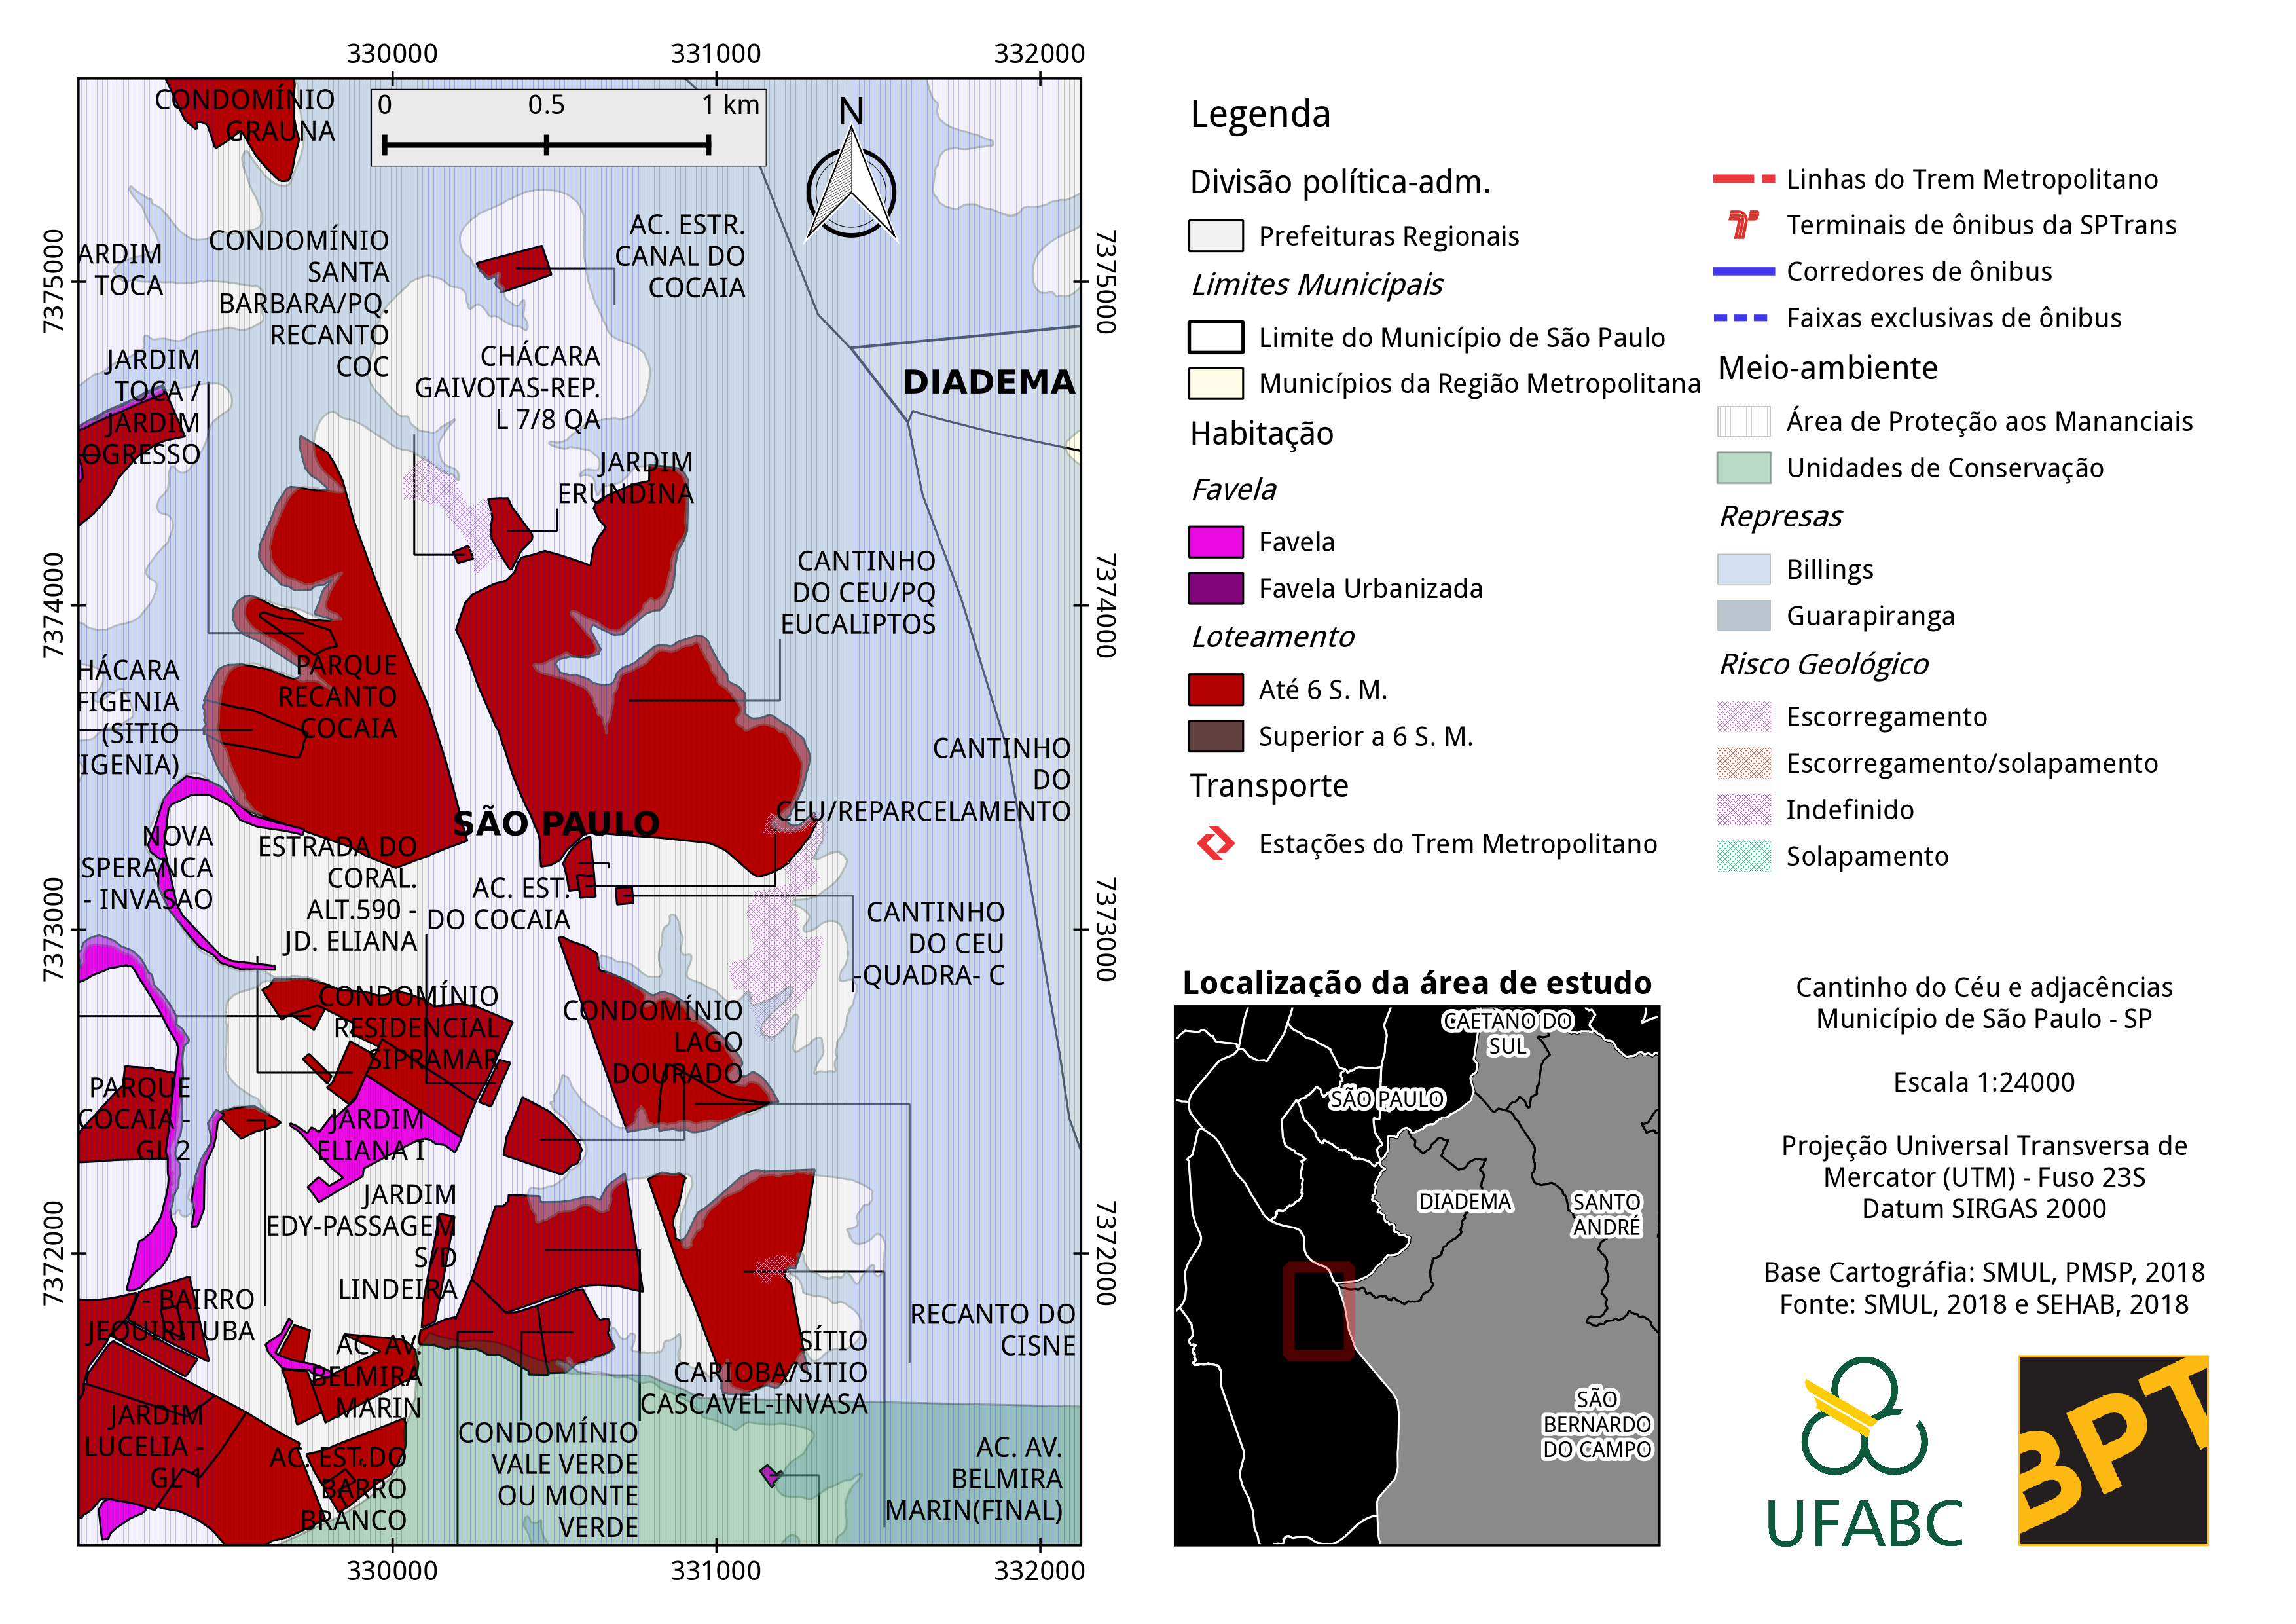
\includegraphics[height=14cm,keepaspectratio]{img/mapa_1-24000}
			\label{fig:mapa_1-24000}
			\legend{Elaboração própria}
		\end{figure}
	\end{landscape}

	\begin{landscape}
		\begin{figure}
			\centering
			\caption{Cantinho do Céu e Adjacências (escala 1:8400)}
			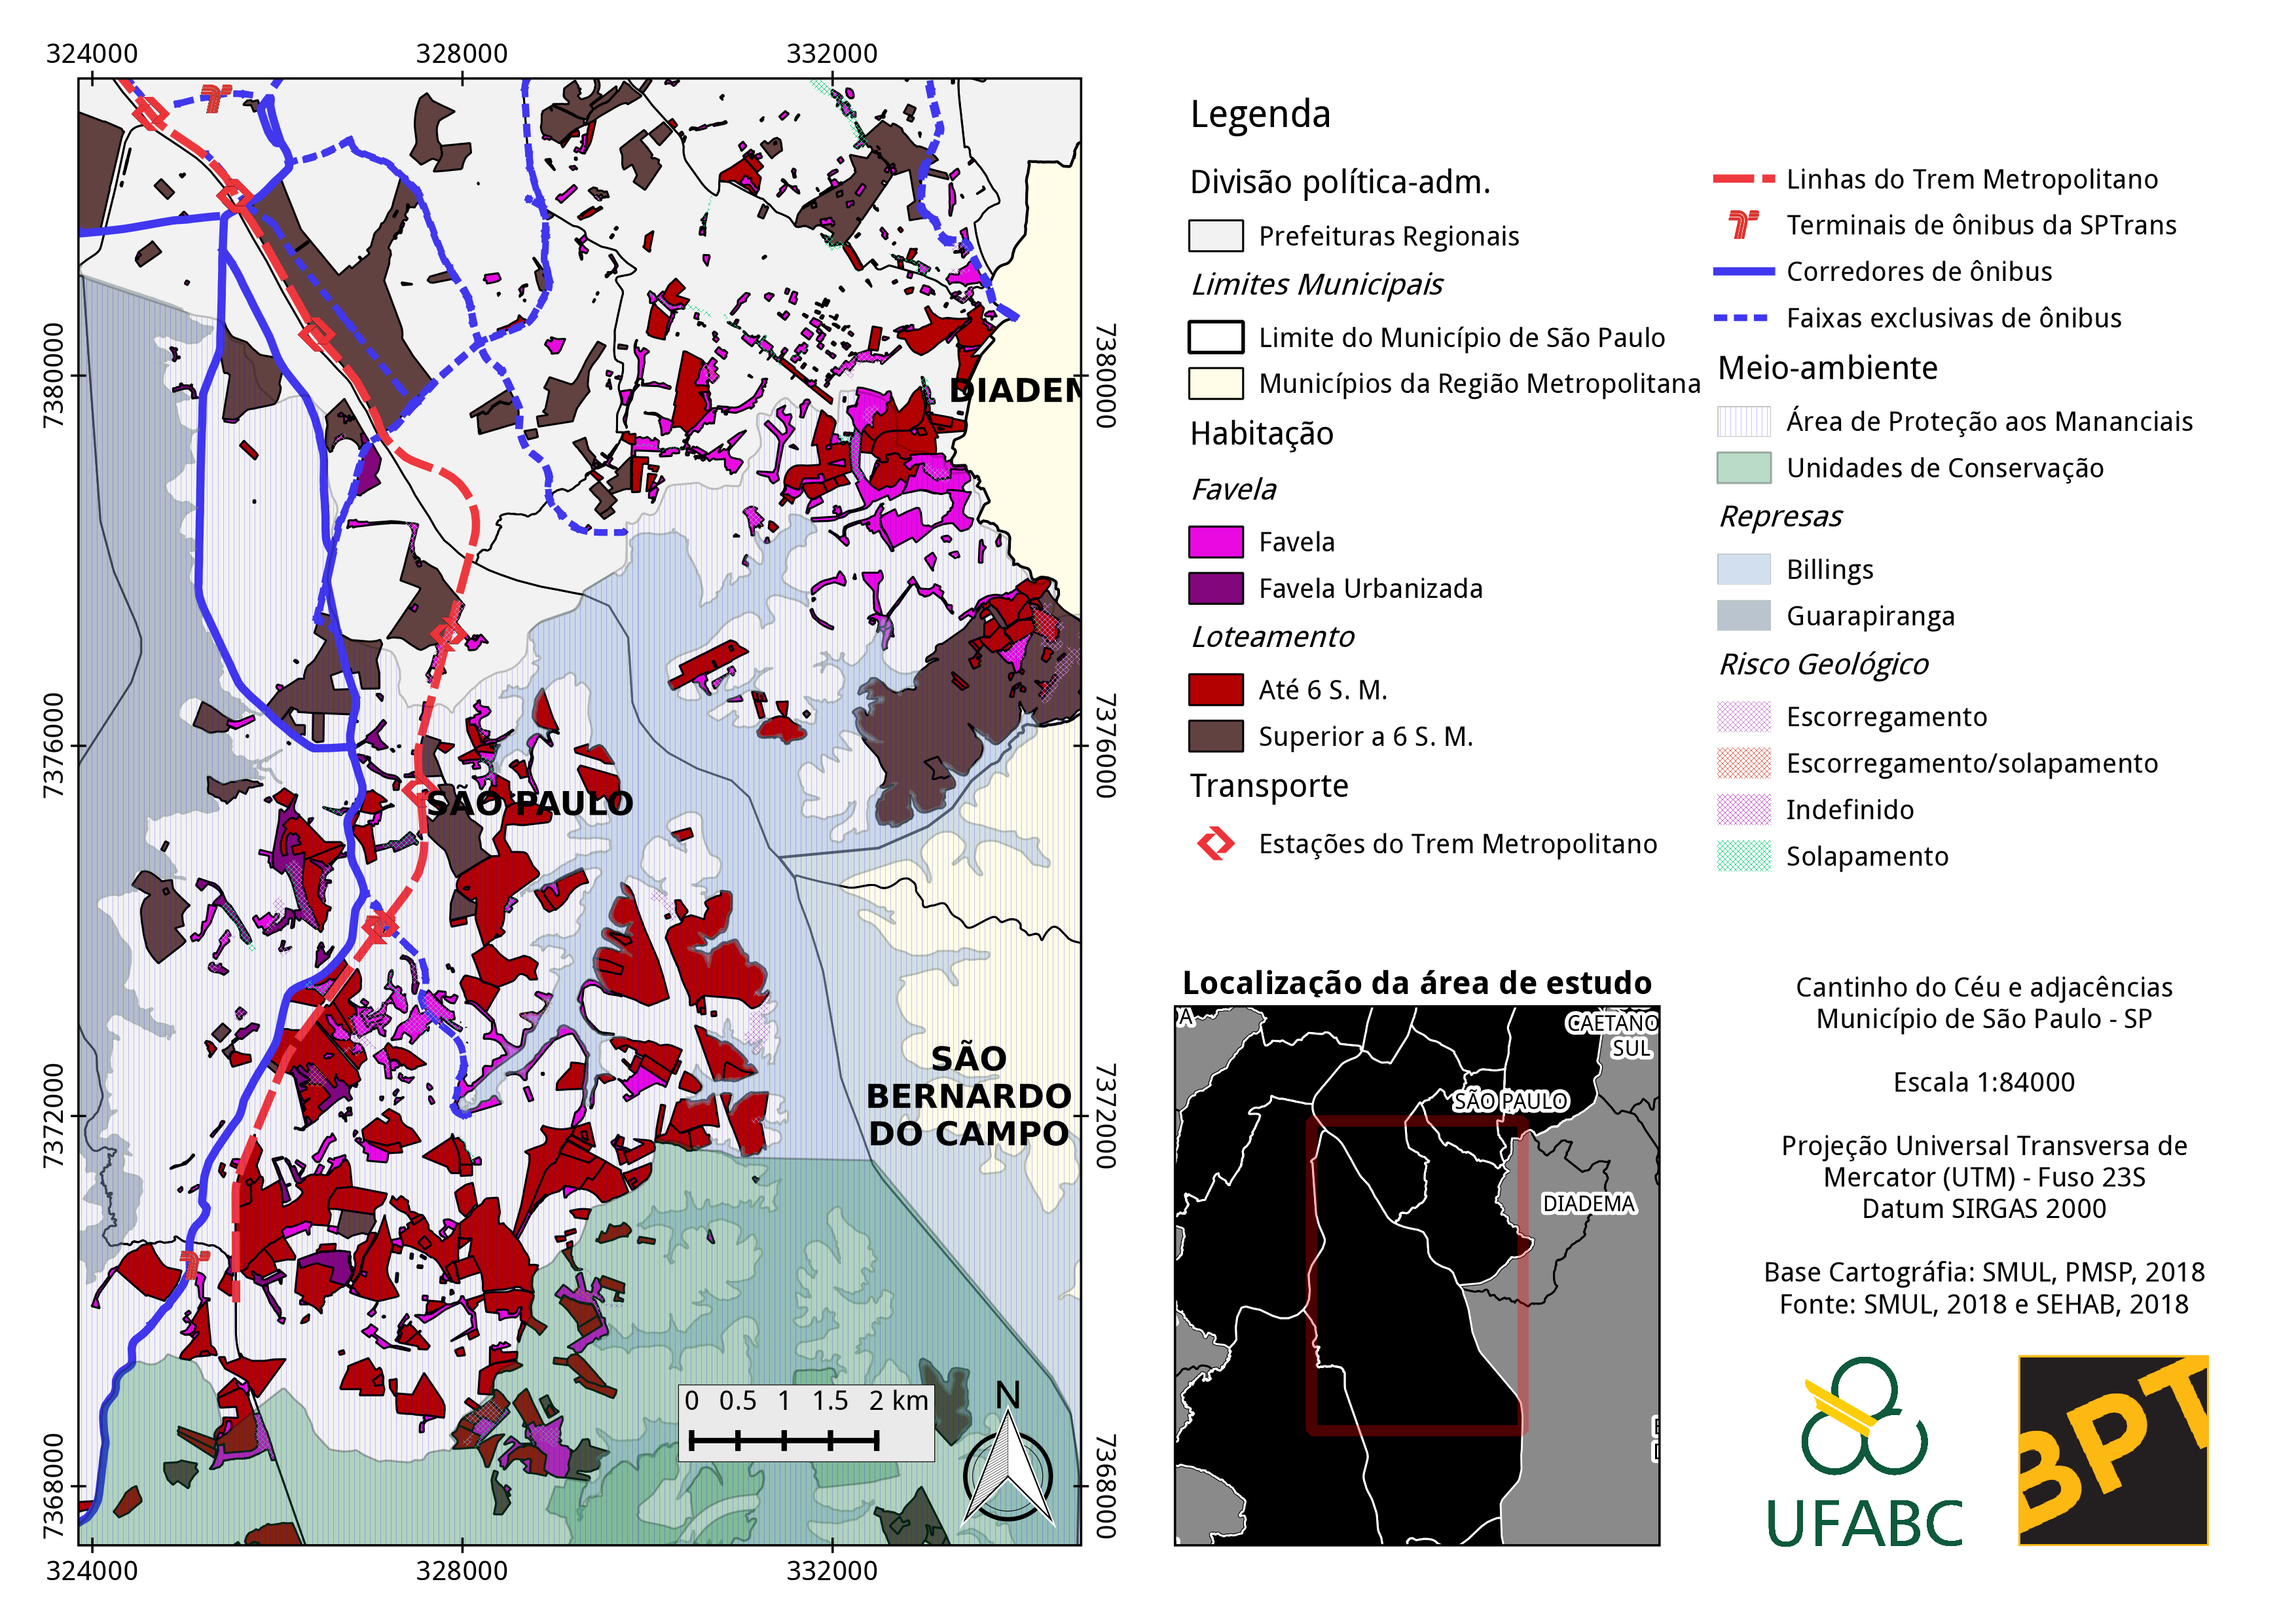
\includegraphics[height=14cm,keepaspectratio]{img/mapa_1-84000}
			\label{fig:mapa_1-84000}
			\legend{Elaboração própria}
		\end{figure}
	\end{landscape}
	
	% TODO (Caio, aqui talvez seja interessante você colocar algumas informações que julgar interessantes sobre os mapas)
	
	A área Cantinho do Céu é composta por dois tipos de ocupação: parcelamento irregular e ocupação desordenada típica de favela. Além disso, o tamanho médio da família do Cantinho do Céu é de 3,44 pessoas por família, o que representa uma média ligeiramente superior à do município de São Paulo (3,3) \cite{Barda2012}.
	
	\begin{figure}[htb]
		\centering
		\caption{Imagem aérea da área do Cantinho do Céu}
		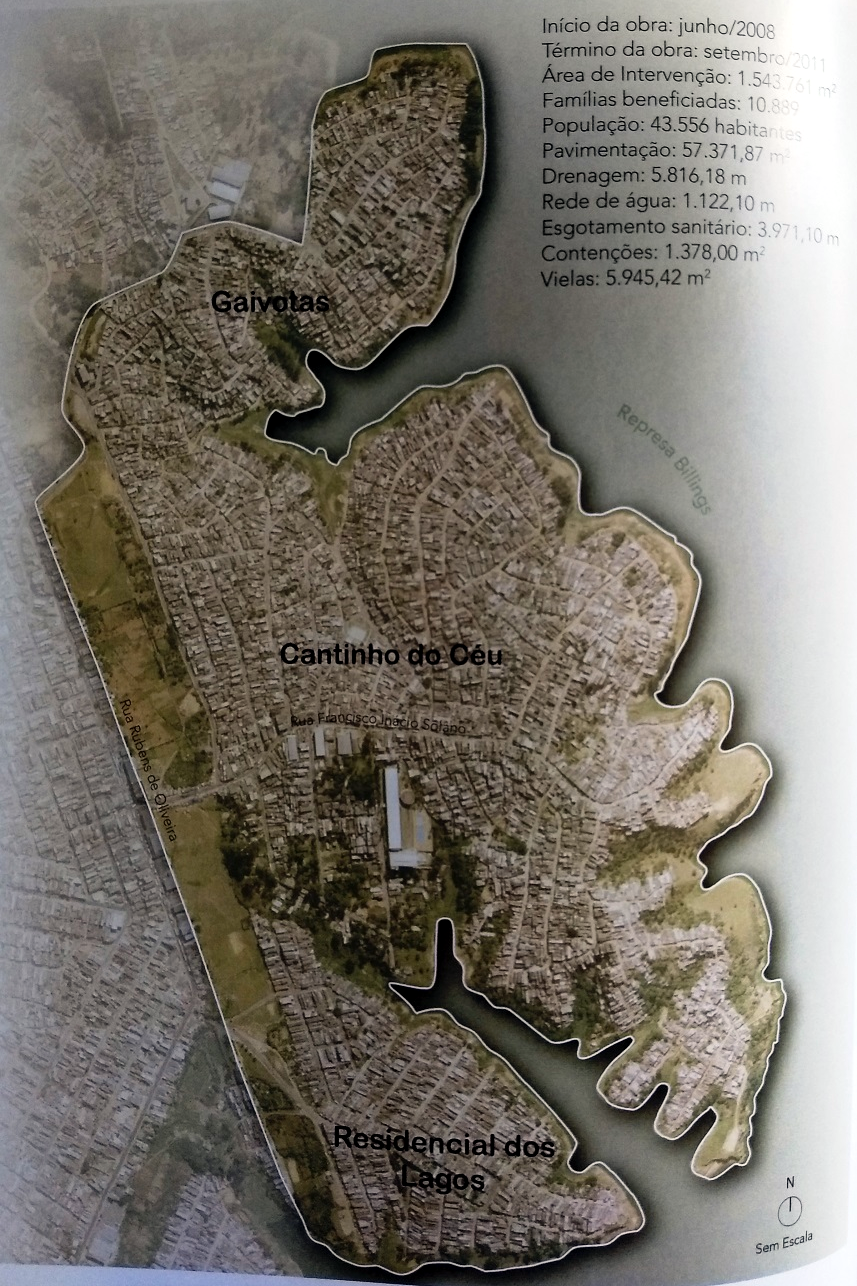
\includegraphics[height=15cm]{img/barda_peninsula}
		\label{fig:peninsula}
		\legend{Fonte: \citeonline{Barda2012}}
	\end{figure}
	
	Os dados mostrados na figura \ref{fig:peninsula}, que mostra como está estabelecida a área do Cantinho do Céu, são reproduzidos abaixo para facilitar sua observação:
	
	\begin{itemize}
	    \item Início da obra: junho/2008;
	    \item Término da obra: setembro/2011;
	    \item Área de intervenção: 1.543.761 m²;
	    \item População: 43.556 habitantes;
	    \item Pavimentação: 57.371,87 m²;
	    \item Drenagem: 5.816,18 m;
	    \item Rede de água: 1.122,10 m;
	    \item Esgotamento sanitário: 3.971,10 m;
	    \item Contenções: 1.378,00 m²;
	    \item Vielas: 5.945,42 m².
	\end{itemize}

	Os desdobramentos que levaram à Urbanização do Cantinho do Céu são muitos, mas como ponto de partida pode ser citado o Programa Guarapiranga, que foi iniciado em 1990, devido à realidade da ocupação irregular das áreas de mananciais. O programa foi constituído por um conjunto de intervenções de infraestrutura.
	
	Em 1997, teve início a terceira etapa da primeira fase do Programa Guarapiranga, mesmo ano em que era aprovada a nova legislação de proteção dos mananciais (Lei Estadual nº 9.866/97), a qual estabelecia o Plano Emergencial, permitindo que os órgão públicos, como a Sabesp e as prefeituras implantassem ações de saneamento básico na região dos mananciais sul, desde que os bairros fizessem parte da lista de áreas precárias publicadas na legislação.
	
	O Plano Emergencial produziu rápida manifestação de lideranças da região Billings, exigindo que as ações do programa de urbanização se estendessem para seus bairros. Duas das lideranças mais ativas eram do Cantinho do Céu e do Jardim Gaivotas, que participavam ativamente das reuniões do subcomitê da bacia Billings.
	
	Como resposta às demandas da população por soluções para atenuar as condições precárias dos bairros irregulares da região, a \gls{sehab} preparou o Programa Billings Legal, buscando recursos financeiros para sua execução e a integração das ações com o Governo do Estado.
	
	No diagnóstico elaborado em função do programa, ficou claro que a área do Cantinho do Céu era uma das mais carentes da cidade de São Paulo e tinha como condição crítica seu esgotamento sanitário, que era efetuado por meio de fossas negras, sujeitas a extravasões frequentes para as valas de drenagem irregulares de águas pluviais.
	
	Em 2005, o Programa Billings Legal foi retomado com o nome de Programa Mananciais, inicialmente uma parceria entre os governos municipal e estadual e, a partir de 2010, com recursos do governo federal. Nesse momento, a \gls{sehab} deu início à elaboração do novo projeto para o Cantinho do Céu, em parceria com a equipe técnica do Ministério Público, com o objetivo de promover uma recuperação ambiental na área mantendo a maioria das famílias que viviam no local.
	
	Finalizado o projeto básico, foi dado início ao processo de contratação da obra e, em 2010, dez anos depois dos primeiros estudos, o canteiro de obras e as máquinas se instalaram no Cantinho do Céu. \cite{Barda2012}
	
	Os eventos acima descritos encontram-se sumarizados na figura \ref*{fig:cronologia}.
	
	\begin{figure}[H]
		\centering
		\caption[Cronologia do surgimento do Cantinho do Céu]{Breve diagrama de eventos cronológicos que desencadearam no surgimento do Cantinho do Céu}
		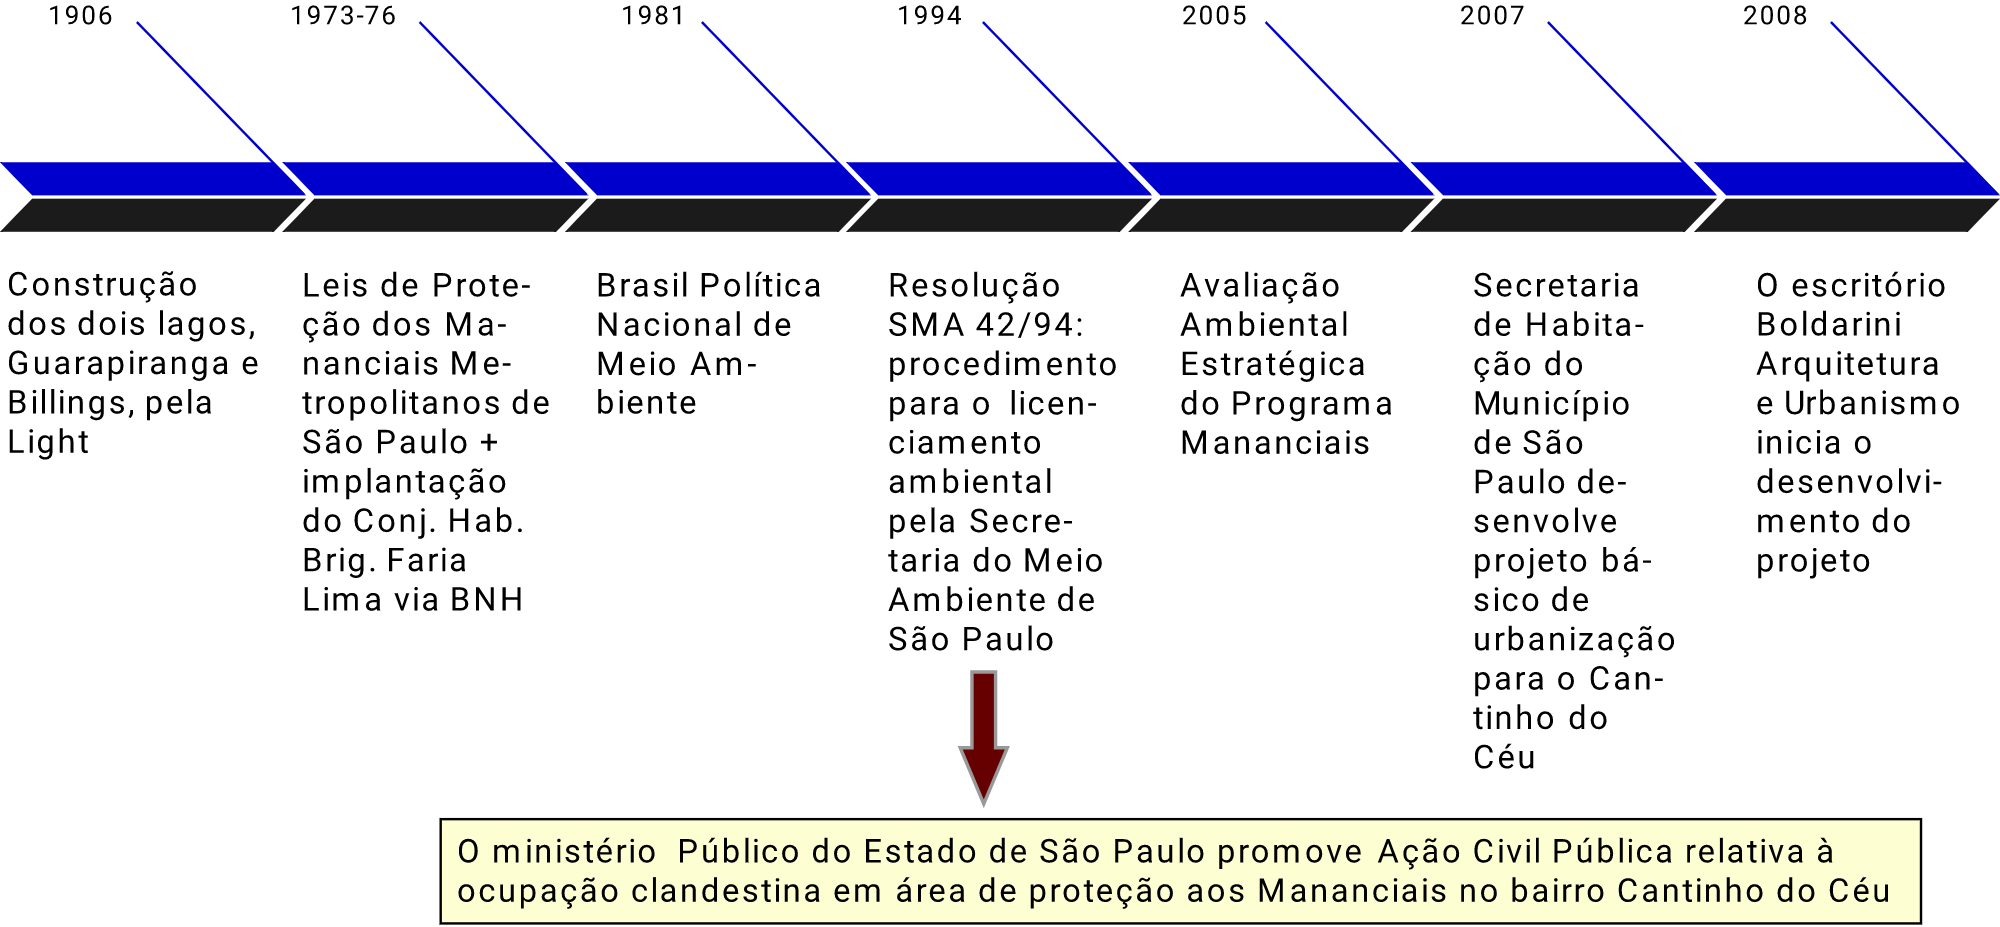
\includegraphics[height=7cm]{img/cronologia}
		\label{fig:cronologia}
		\legend{Elaboração própria com base em \citeonline{Barda2012}}
	\end{figure}
	
	As figuras \ref{fig:fotos_antes_01}, \ref{fig:fotos_antes_02} e \ref{fig:fotos_antes_03} mostram o Cantinho do Céu antes do programa de urbanização. Como características marcantes, pode-se observar a proximidade de construção de algumas residências à represa, as ruas de terra e a ausência de vias que possibilitem a ligação de todas as áreas do bairro.
	
	\begin{figure}[p]
		\centering
		\caption{Cantinho do Céu antes da urbanização}
		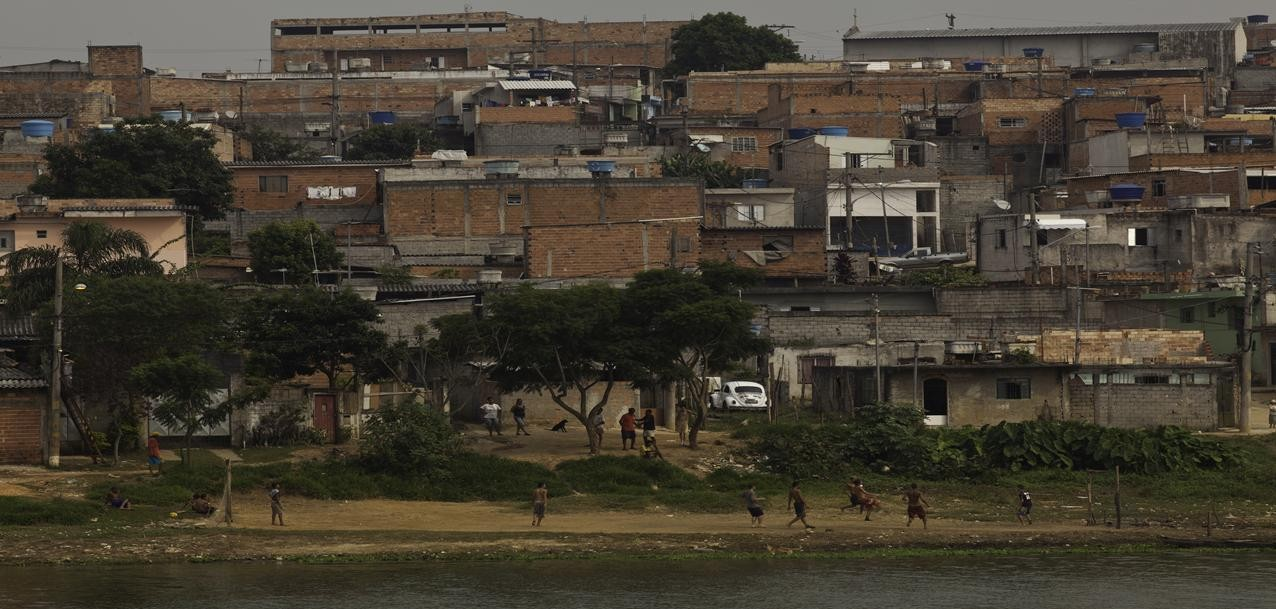
\includegraphics[width=0.5\textwidth]{img/knoll_antes01}
		\label{fig:fotos_antes_01}
		\legend{Fonte: \citeonline{Archdaily2013}, direitos reservados a Fábio Knoll}
	\end{figure}
	
	\begin{figure}[p]
		\centering
		\caption{Cantinho do Céu antes da urbanização}
		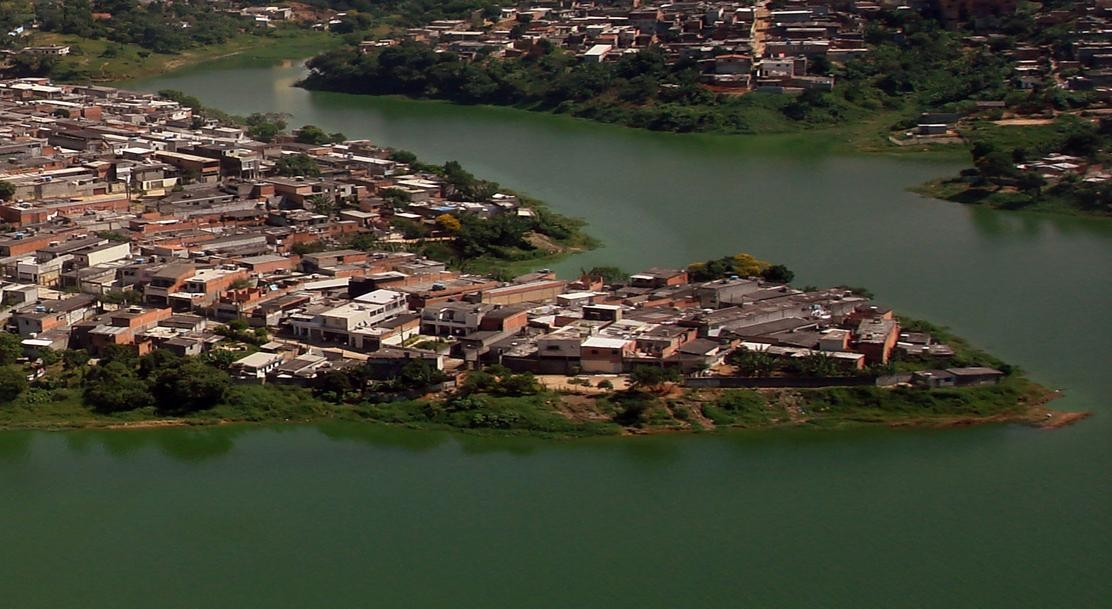
\includegraphics[width=0.5\textwidth]{img/knoll_antes02}
		\label{fig:fotos_antes_02}
		\legend{Fonte: \citeonline{Archdaily2013}, direitos reservados a Fábio Knoll}
	\end{figure}
	
	\begin{figure}[p]
		\centering
		\caption{Cantinho do Céu antes da urbanização}
		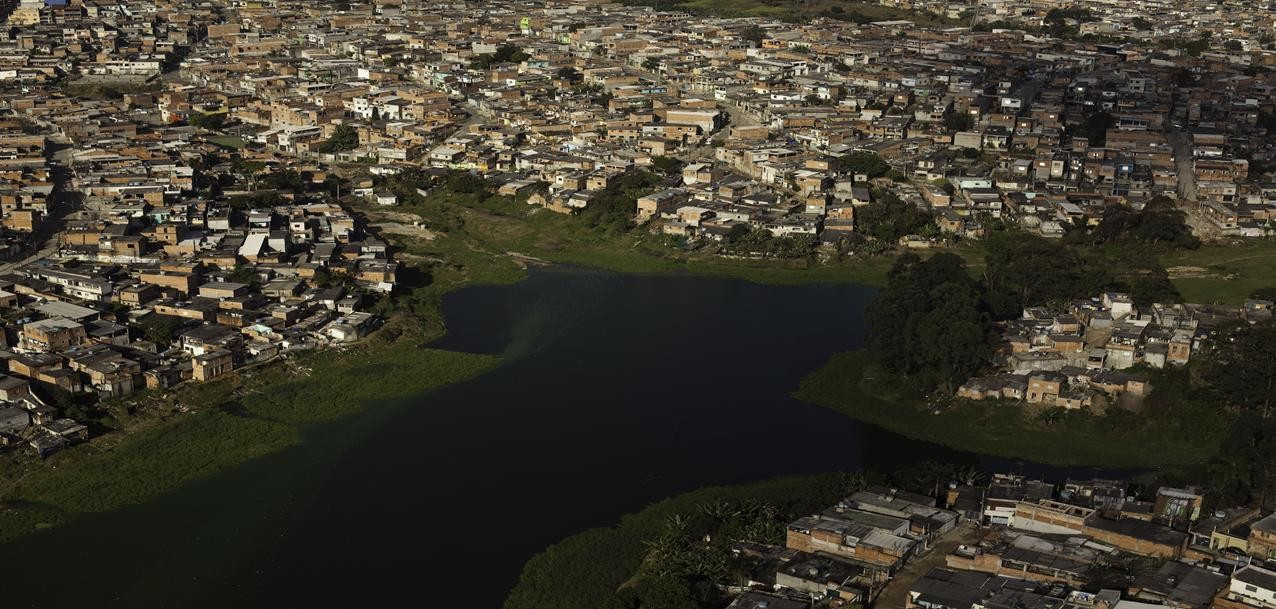
\includegraphics[width=0.5\textwidth]{img/knoll_antes03}
		\label{fig:fotos_antes_03}
		\legend{Fonte: \citeonline{Archdaily2013}, direitos reservados a Fábio Knoll}
	\end{figure}
	
	\chapter{Projeto de intervenção}
	O projeto de atuação no Cantinho do Céu se inicia no ano de 2008, tendo uma duração de 04 anos, sendo finalizado ao final do ano de 2012. Porém, o projeto tem uma data de inicio muito anterior a de 2008. 
	
	A primeira ação que se tem tomada sobre a região data de 2002, quando a Secretaria da Habitação recebe uma ordem judicial para realizar a desocupação de toda a região em 30 dias. Devido a grande quantidade de pessoas que haveriam de ser removidas, aproximadamente 20 mil habitantes, a proposta de remoção torna-se inviável, dando início a diálogos junto ao Ministério Público para o desenvolvimento de outras alternativas para solução do problema habitacional da região.
	
	Em 2005 começa-se a traçar um plano de correção com vistas a manter a população que ali vivia, fornecendo a área toda a estrutura necessária \cite{Barda2012}.
	
	No ano de 2008 o escritório de Arquitetura  Boldarini Arquitetura e Urbanismo inicia as obras de intervenção sobre a região.
	
	\section{Objetivo do projeto}
	
	O objetivo do projeto era propor uma urbanização adequada sobre toda a região do Cantinho do Céu, dotando-o de toda a infraestrutura necessária, permitindo o desenvolvimento de sua população como indivíduo e sociedade. Dentre todas as ações necessárias, pode-se citar algumas ações tomadas como estratégias de intervenção, sendo elas \cite{Barda2012}:
	
	\begin{itemize}
	    \item Preservação da vida, realizando correções em todas as áreas/habitações identificadas que apresentavam risco a segurança e saúde da população;
	    \item Integração urbanísticas entre as novas intervenções, permitindo o acesso as demais áreas, respeitando a tipologia de cada região;
	    \item Correção na infraestrutura urbana, adequando e implementando redes de esgoto, realizando melhorias ambientais e ampliação da malha rodoviária ;
	    \item Geração de condições para a realização da regularização fundiária de todos os integrantes da região.
	\end{itemize}
	
	% Caio, favor inserir imagem aqui!
	
	\section{Dificuldades encontradas}
	
	Como todo o projeto de intervenção e adequação de favelas, o projeto Cantinho do Céu também apresentou dificuldade de concepção durante todo o período de implementação. 
	
	A primeira dificuldade apresentou-se quanto a recepção da própria população do local. Em primeiro momento a população mostrava certa resistência frente ao programa, alegando que não era primeira promessa de melhoria do local e que, como a anterior, também não seria cumprida conforme prometido. Porém, com o avanço do projeto e as melhorias ganhando destaque na região, a população passa a aceitar mais ao programa e a interagir mais com as equipes, aumentando a aproximação entre as partes.
	
	Quanto à região, o projeto enfrentou dificuldade a respeito de sua topologia devido a sua declividade acentuada e a desordenada implementação que ocorrera no bairro ao longo dos anos. Estes fatores dificultaram o processo de implementação das redes de esgoto e da malha viária. Para a realização desta atividade foi necessário que cerca de 10\% das família fossem removidas para outras regiões, permitindo o acesso e início de obras. 
	
	Por fim ressalta-se a dificuldade frente aos órgãos públicos para a concepção do projeto. Para a realização da intervenção, se fez necessário integração da Secretaria do Verde e Meio Ambiente, secretaria da Educação e Saúde; do Governo do Estado participaram a Secretaria de Saneamento, Secretaria de Meio Ambiente e Sabesp. Segundo Ricardo Sampaio, engenheiro integrante da equipe de intervenção, realizar o trabalho integrado entre todos os órgãos e secretarias atuantes sobre o projeto mostrou-se como um dos maiores desafios enfrentados pela equipe \cite{Barda2012}.
	
	\section{Algumas soluções adotadas}
	
	\chapter{Situação atual}
	
	Conforme \citeonline[p.114]{Silva2016}:
	
	\begin{citacao}
	    ``A construção do parque linear prevê que ele seja feito em toda a orla da Península do Ribeirão Cocaia, e por enquanto foi feito uma parte de apenas 1,5 km da orla da Península. A política possui a ideia de desfazimento, que é um conceito que a prefeitura do município de São Paulo vinha aplicando durante a gestão Kassab, que previa entre outras coisas a remoção de pessoas que encontravam-se próximos à borda da represa (\dots)''
    \end{citacao}
	
	Para \citeonline[p.120]{Silva2016}:
	
	\begin{citacao}
	   ``O parque linear em si não é o problema, nem tampouco soluciona o problema. No máximo, ele poderia ser parte da solução, uma vez que desapropriar e fazer o parque pode resolver um problema pontual; porém, sem o encaminhamento adequado para a questão habitacional não há como resolver a situação da área de proteção de mananciais.''
	\end{citacao}
	
	\section{Visita de campo}
	
	%===============================================================================
	%
	
	% ----------------------------------------------------------
	% ----------------------------------------------------------
	\postextual
	
	
	
	% informa o arquivo com a bibliografia. Deve ser o mesmo nome
	% (sem o sufixo) que será informado no ambiente filecontents
	% que está no final deste arquivo. Neste exemplo foi usado 
	% bibitemp.bib e bibtemp. Este comando insere a bibliografia
	% nesta posição (antes dos apêndices, anexos, índice remissivo)
	\bibliography{fontes}
	% ----------------------------------------------------------
	% Glossário
	% ----------------------------------------------------------
	% Consultar manual da classe abntex2 para orientações sobre o
	% uso do glossário.
	\renewcommand{\glossaryname}{Glossário}
	%\renewcommand{\glossarypreamble}{Esta é a descrição do glossário.\\ \\}
	\renewcommand*{\glsseeformat}[3][\seename]{\textit{#1}
		\glsseelist{#2}}
	
	% ---
	% Traduções para o ambiente glossaries
	% ---
	\providetranslation{Glossary}{Glossário}
	\providetranslation{Acronyms}{Siglas}
	\providetranslation{Notation (glossaries)}{Notação}
	\providetranslation{Description (glossaries)}{Descrição}
	\providetranslation{Symbol (glossaries)}{Símbolo}
	\providetranslation{Page List (glossaries)}{Lista de Páginas}
	\providetranslation{Symbols (glossaries)}{Símbolos}
	\providetranslation{Numbers (glossaries)}{Números} 
	% ---
	
	% ---
	% Imprime o glossário
	% ---
	\cleardoublepage
	\phantomsection
	\addcontentsline{toc}{chapter}{\glossaryname}
	% \glossarystyle{index}
	% \glossarystyle{altlisthypergroup}
	\glossarystyle{tree}
	\printglossaries
	% ---
	
	% ----------------------------------------------------------
	% Apêndices
	% ----------------------------------------------------------
	
	% ---
	% Inicia os apêndices. Não esquecer de fechar ao final de
	% todos os apêndices (\end{apendicesenv})
	% ---
	%\begin{apendicesenv}
	
	% Imprime uma página indicando o início dos apêndices
	%\partapendices
	
	% ----------------------------------------------------------
	%\chapter{Primeiro apêndice}
	% ----------------------------------------------------------
	
	%Este é um exemplo de inclusão de capítulos de %apêndice em uma 
	%monografia.  Cada apêndice é tratado como se fosse %um capítulo.
	%Os apêndices devem ser iniciados pelo comando de %ambiente
	%\textbackslash begin\{apendicesenv\} e encerrados %pelo comando 
	%\textbackslash end\{apendicesenv\}.
	
	% ----------------------------------------------------------
	%\chapter{Segundo apêndice}
	% ----------------------------------------------------------
	
	%Este é um exemplo de inclusão de um segundo apêndice. 
	
	%\end{apendicesenv}
	% ---
	
	
	% ----------------------------------------------------------
	% Anexos
	% ----------------------------------------------------------
	
	% ---
	% Inicia os anexos
	% ---
	%\begin{anexosenv}
	
	% Imprime uma página indicando o início dos anexos
	%\partanexos
	
	% ---
	%\chapter{Anexo I}
	% ---
	%Os anexos são similares aos apêndices se distinguindo pelo fato
	%que os apêndices são de autoria do autor da monografia e os 
	%anexos não são da autoria do autor da monografia.  Por exemplo,
	%se incluir no trabalho um modelo de um formulário preenchido
	%por alunos participantes de uma pesquisa, este será um apêndice
	%se o formulário foi criado pelo autor da monografia e será um
	%anexo se o formulário tiver sido criado por outros (por exemplo,
	%é um formulário padrão da escola em que o aluno que o preenche
	%estuda).
	%
	%Mesmo que o formulário tenha sido elaborado pela escola, uma
	%reprodução do formulário preenchido por cada aluno na pesquisa
	%será incluído no apêndice pois envolve o trabalho do autor da
	%monografia ao distribuir, coletar e reproduzir as respostas.
	%
	%Este é um exemplo de inclusão de capítulos de anexos em uma 
	%monografia.  Cada anexo é tratado como se fosse um capítulo.
	%Os anexos devem ser iniciados pelo comando de ambiente
	%\textbackslash begin\{anexoenv\} e encerrados pelo comando 
	%\textbackslash end\{anexoenv\}.
	%
	%\end{anexosenv}
	% ---
	%---------------------------------------------------------------------
	%---------------------------------------------------------------------
	
	%\printindex
	
	% Por padrão são incluídas no trabalho somente as referências
	% citadas ao longo do texto. No comando abaixo foram acrescentadas
	% algumas referências não citadas (neste texto servem apenas como
	% exemplos). Não deve ser usado o comando (mais simples) 
	% \nocite{*}, pois este parece não ser compatível com o
	% abntex2cite
	%\nocite{abntex2cite,abntex2wiki,boyer,eves,iezzi,kletenic,
	%        diomara,steinbruch,intusolatex,feynman,shannon,
	%        luisfelipe,turing}
\end{document}
